
\documentclass[12pt,a4paper]{article}

% Configuracion del idioma
\usepackage[utf8]{inputenc}
\usepackage[T1]{fontenc}
\usepackage[spanish,es-noshorthands]{babel}


% Formato de pagina
\usepackage[a4paper,margin=2.5cm]{geometry}
\usepackage{setspace}
\onehalfspacing

% Enlaces
\usepackage[hidelinks]{hyperref}

% Graficos e imagenes
\usepackage{graphicx}
\usepackage{float}

% Citas bibliograficas
\usepackage[style=apa,backend=biber]{biblatex}
\usepackage{csquotes}
\addbibresource{referencias.bib}



\begin{document}
	
	
	\begin{titlepage}
		\centering
		
		\vspace*{2cm}
		
		{\Large Universidad Politécnica de Pachuca\par}
		
		\vspace{2cm}
		
		{\huge\bfseries Tecnologías para el desarrollo de aplicaciones 
			móviles\par}
		
		\vspace{0.5cm}
		
		{\Large Estudio y aplicación de herramientas para 
			el desarrollo en Android\par}
		
		\vspace{2cm}
		
		
		
		\begin{flushleft}
			\textbf{Asignatura:} Aplicaciones Móviles
			
			\vspace{0.5cm}
			
			\textbf{Estudiante:} Guillermo Ruiz Marquez
			
			\vspace{0.5cm}
			
			\textbf{Profesor:} Miguel Angel Montoya Cerro 
		\end{flushleft}
		
		\vfill
		
		Pachuca, Hidalgo, Mexico\\
		\today
		
	\end{titlepage}
	%Tabla de contenidos
	\tableofcontents
	
	%Indice de figuras 
	\newpage 
	\listoffigures
	
	%%Indice de tablas
	\newpage 
	\listoftables

	%introduccion
	\newpage

\section{Introducción}

El desarrollo de aplicaciones móviles ha adquirido una gran
importancia dentro de la industria del software, debido a la
necesidad de crear herramientas digitales que permitan realizar
diferentes actividades desde dispositivos como teléfonos
inteligentes y tabletas. Para llevar a cabo este tipo de
desarrollos es necesario conocer los lenguajes de programación,
los entornos de desarrollo y las tecnologías que permiten
construir, ejecutar y probar aplicaciones.

En este contexto, el desarrollo de aplicaciones para el sistema
operativo Android requiere el uso de diferentes herramientas y
tecnologías. Entre ellas se encuentran Android Studio como entorno
de desarrollo integrado, Kotlin como lenguaje de programación y
Jetpack Compose como herramienta para la construcción de
interfaces de usuario. Cada una cumple una función específica
dentro del proceso de desarrollo y permite trabajar en diferentes
aspectos de una aplicación móvil.

El presente documento tiene como propósito describir y analizar
las tecnologías y herramientas utilizadas durante las prácticas
de la asignatura de Aplicaciones Móviles. A través de las
actividades realizadas se busca comprender su funcionamiento,
identificar sus principales características y explicar su
utilización mediante ejemplos y ejercicios prácticos.

Asimismo, se documentarán los procedimientos realizados en cada
práctica, incluyendo explicaciones, fragmentos de código y
capturas de pantalla que permitan observar tanto el uso de las
herramientas como los resultados obtenidos. De esta manera, el
documento servirá como evidencia del aprendizaje y de los
conocimientos adquiridos durante el estudio de las tecnologías
para el desarrollo de aplicaciones móviles.

\section{Planteamiento del problema}

El desarrollo de aplicaciones móviles requiere el conocimiento y
la utilización de diferentes tecnologías, herramientas y
lenguajes de programación que permiten construir soluciones
digitales para dispositivos móviles. Sin embargo, para comprender
este proceso no basta con conocer los conceptos teóricos, sino
que también es necesario experimentar con los entornos de
desarrollo, identificar sus funciones y aplicar sus herramientas
mediante ejercicios prácticos.

En este contexto, resulta importante conocer las tecnologías
utilizadas para el desarrollo de aplicaciones en el sistema
operativo Android, así como comprender la relación que existe
entre el entorno de desarrollo, el lenguaje de programación y
las herramientas destinadas a la construcción de interfaces
de usuario.

Por lo anterior, se plantea la necesidad de estudiar y
documentar las características, funciones y procedimientos de
las tecnologías utilizadas durante las prácticas de la
asignatura de Aplicaciones Móviles, con el propósito de
comprender su funcionamiento y reconocer su aplicación dentro
del proceso de desarrollo de software.

\section{Objetivo general}

Analizar y aplicar las principales tecnologías y herramientas
utilizadas para el desarrollo de aplicaciones móviles en
Android, mediante actividades prácticas que permitan
comprender sus características, funciones y procedimientos
de utilización.	

\section{Objetivos específicos}

\begin{enumerate}
	\item Identificar las características y funciones de los
	entornos de desarrollo utilizados para crear aplicaciones
	móviles.
	
	\item Comprender los fundamentos del lenguaje de
	programación Kotlin y su utilización en el desarrollo
	de aplicaciones Android.
	
	\item Explorar las herramientas y componentes de
	Jetpack Compose para la construcción de interfaces
	de usuario.
	
	\item Aplicar los conocimientos adquiridos mediante
	ejercicios y actividades prácticas.
	
	\item Documentar los procedimientos realizados,
	describiendo las herramientas utilizadas y los
	resultados obtenidos.
	
	\item Reconocer la importancia de las tecnologías
	estudiadas dentro del proceso de desarrollo de
	aplicaciones móviles.
\end{enumerate}


\section{Justificación}

Desde una perspectiva académica, el estudio de las tecnologías
para el desarrollo de aplicaciones móviles permite adquirir
conocimientos sobre las herramientas y procedimientos
necesarios para construir software destinado a dispositivos
móviles. La realización de prácticas facilita la comprensión
de los conceptos teóricos mediante su aplicación en ejercicios
que permiten observar el funcionamiento de cada herramienta.

Desde una perspectiva tecnológica, conocer entornos de
desarrollo como Android Studio, lenguajes como Kotlin y
herramientas como Jetpack Compose permite comprender los
elementos que intervienen en la creación de aplicaciones
para Android. Asimismo, su utilización proporciona experiencia
en la escritura de código, la construcción de interfaces y
la visualización de resultados.

Finalmente, la documentación de las prácticas permite
registrar los procedimientos realizados, explicar las
características de las herramientas utilizadas y presentar
evidencias de los resultados obtenidos. De esta manera, el
documento constituye un registro del aprendizaje y de los
conocimientos adquiridos durante la asignatura.

\section{Alcance y limitaciones}

El presente trabajo comprende el estudio y la aplicación
de tecnologías y herramientas utilizadas en el desarrollo
de aplicaciones móviles para el sistema operativo Android.
Se abordarán los conceptos y procedimientos presentados
durante las prácticas de la asignatura, considerando el uso
del entorno de desarrollo, el lenguaje de programación y
las herramientas para la construcción de interfaces.

El alcance del documento se limita a las tecnologías,
funciones y procedimientos revisados durante las actividades
académicas. Por lo tanto, no pretende abarcar la totalidad
de las herramientas disponibles para el desarrollo de
aplicaciones móviles ni profundizar en tecnologías que no
formen parte de las prácticas realizadas.

\subsection{Estructura del documento}

El presente documento se encuentra organizado en diferentes
apartados que permiten presentar los fundamentos teóricos
y las actividades prácticas relacionadas con el desarrollo
de aplicaciones móviles.

En primer lugar, se presenta la introducción, donde se
describe el contexto del trabajo, el planteamiento del
problema, los objetivos, la justificación y el alcance.

Posteriormente, se desarrolla el marco teórico, en el que
se explican los conceptos y fundamentos de las tecnologías
y herramientas relacionadas con el desarrollo de
aplicaciones móviles.

A continuación, se presenta el desarrollo, organizado
en diferentes prácticas. En cada una se describen las
herramientas utilizadas, sus características, los
procedimientos realizados y los resultados obtenidos,
acompañados de las evidencias correspondientes.

Finalmente, se incluyen las conclusiones, los anexos y
las referencias bibliográficas utilizadas para la
elaboración del documento.

\section{Marco teórico}
\subsection{Aplicaciones moviles}
Las aplicaciones móviles son programas de software diseñados
para ejecutarse en dispositivos móviles, como teléfonos
inteligentes y tabletas. Estas aplicaciones permiten realizar
diferentes actividades mediante una interfaz de usuario que
facilita la interacción con las funciones y herramientas
disponibles.

Entre sus características se encuentran la portabilidad,
la accesibilidad y la posibilidad de ofrecer diferentes
funcionalidades de acuerdo con las necesidades de los
usuarios. Además, pueden utilizar los recursos y
componentes del dispositivo para proporcionar servicios
y herramientas que faciliten distintas actividades.

El desarrollo de aplicaciones móviles comprende diferentes
etapas y requiere el uso de lenguajes de programación,
entornos de desarrollo y herramientas especializadas.
Estas tecnologías permiten diseñar interfaces, implementar
funcionalidades, administrar información y realizar pruebas
para comprobar el funcionamiento de las aplicaciones.


\subsection{Sistema operativo Android}
Android es un sistema operativo diseñado principalmente para
dispositivos móviles, como teléfonos inteligentes y tabletas.
Proporciona un entorno en el que se pueden ejecutar
aplicaciones y ofrece diferentes herramientas y componentes
que permiten a los desarrolladores crear programas para
esta plataforma.

El desarrollo de aplicaciones para Android puede realizarse
mediante diferentes lenguajes de programación, como Kotlin
y Java, utilizando las herramientas y bibliotecas disponibles
en el entorno de desarrollo. Las aplicaciones utilizan
componentes que permiten organizar su funcionamiento y
gestionar la interacción con el sistema operativo.

De acuerdo con Android Developers, entre los componentes
principales de las aplicaciones Android se encuentran las
actividades, los servicios, los receptores de emisiones y
los proveedores de contenido \textcite{androidSistema}.
Estos elementos permiten estructurar las diferentes
funciones que puede realizar una aplicación.

Android también proporciona un conjunto de herramientas
y recursos para facilitar el desarrollo, la ejecución y
la depuración de aplicaciones. Su ecosistema permite
integrar diferentes tecnologías y bibliotecas que ayudan
a los desarrolladores a implementar las funcionalidades
de sus aplicaciones.


\subsection{Lenguaje de programacion Kotlin}
Kotlin es un lenguaje de programación de tipado estático
que permite desarrollar aplicaciones para diferentes
plataformas. El tipado estático significa que los tipos
de datos de las variables se determinan durante la
compilación, lo que permite detectar determinados
errores antes de ejecutar el programa.

Este lenguaje se caracteriza por ofrecer una sintaxis
concisa y herramientas que facilitan la escritura y el
mantenimiento del código. Además, cuenta con
compatibilidad con Java y proporciona características
que permiten desarrollar aplicaciones para el sistema
operativo Android.

Android Developers destaca la integración de Kotlin
con las herramientas y bibliotecas de desarrollo de
Android, así como su compatibilidad con las tecnologías
utilizadas en esta plataforma
\textcite{androidKotlinDocs}.

Kotlin permite implementar la lógica de las aplicaciones
mediante funciones, clases, variables y estructuras de
control. También ofrece características como la
inferencia de tipos, las funciones de extensión y el
manejo de valores nulos, que contribuyen a la
organización y seguridad del código.

\subsection{Jetpack Compose}
Jetpack Compose es un conjunto de herramientas moderno
para desarrollar interfaces de usuario en aplicaciones
Android. Utiliza un enfoque declarativo, mediante el cual
los desarrolladores describen cómo debe mostrarse la
interfaz de acuerdo con el estado de la aplicación, en
lugar de modificar manualmente cada elemento visual.

Una de sus principales características es el uso de
funciones composables, las cuales permiten construir y
organizar los elementos que forman parte de una interfaz.
Estas funciones pueden combinarse para crear componentes
reutilizables, facilitando el desarrollo y mantenimiento
de las pantallas de una aplicación.

De acuerdo con Android Developers, Jetpack Compose
permite desarrollar interfaces de usuario utilizando
Kotlin y ofrece herramientas para administrar los cambios
visuales conforme se modifica el estado de la aplicación
\textcite{androidComposeDocs}.

Jetpack Compose proporciona recursos para organizar
los elementos visuales de una aplicación, crear
componentes reutilizables y definir la distribución de
los elementos en pantalla. Su integración con Kotlin
permite desarrollar interfaces mediante código y
facilita la actualización de los componentes cuando
cambia el estado de la aplicación.



\subsection{Almacenamiento local de datos}

El almacenamiento local de datos permite que una aplicación guarde información directamente en el dispositivo donde se ejecuta, sin depender necesariamente de una conexión a Internet o de un servidor externo. Este mecanismo resulta útil cuando se necesita conservar información estructurada y permitir que el usuario pueda consultarla posteriormente.

En el desarrollo de aplicaciones Android existen diferentes alternativas para almacenar información. Una de ellas es SQLite, un sistema de gestión de bases de datos relacionales que permite organizar los datos mediante tablas y realizar operaciones como insertar, consultar, modificar y eliminar registros.

De acuerdo con Android Developers, Room es una biblioteca de persistencia que proporciona una capa de abstracción sobre SQLite, facilitando el acceso a los datos y reduciendo la necesidad de escribir código repetitivo. Además, permite verificar las consultas SQL durante la compilación y gestionar las modificaciones de la estructura de la base de datos \parencite{androidRoom}.

Room se organiza principalmente mediante tres componentes: las entidades, que representan las tablas donde se almacenan los datos; los objetos de acceso a datos (DAO), que contienen las operaciones para consultar y modificar la información; y la clase de base de datos, que funciona como punto de acceso a los demás componentes.

 

\subsection{Pruebas de software}
Las pruebas de software son una parte fundamental del proceso de desarrollo de una aplicación, ya que permiten comprobar que sus funciones se comportan de acuerdo con los requisitos establecidos. Su propósito es identificar errores, verificar el funcionamiento de los componentes y mejorar la calidad del producto antes de que llegue a sus usuarios.

En el desarrollo de aplicaciones Android se pueden realizar diferentes tipos de pruebas. Entre ellas se encuentran las pruebas unitarias, que permiten verificar el funcionamiento de partes específicas del código; las pruebas de integración, que comprueban la interacción entre distintos componentes; y las pruebas de interfaz de usuario, que permiten verificar que los elementos visuales y las acciones realizadas por el usuario respondan correctamente. Android Developers también señala la importancia de realizar pruebas en emuladores y dispositivos físicos para comprobar el comportamiento de la aplicación en distintos entornos \parencite{androidTesting}.

Además, las pruebas pueden realizarse de forma manual o automatizada. Las pruebas manuales consisten en ejecutar la aplicación e interactuar con sus funciones para identificar posibles problemas. Por otro lado, las pruebas automatizadas utilizan herramientas y código para ejecutar verificaciones de manera repetible, facilitando la detección temprana de errores.

\section{Desarrollo}

\subsection{Practica 1. Jetpack Compose desde cero }

\subsubsection{Introducción}

\subsubsection{Herramientas y tecnologías utilizadas}

\subsubsection{Procedimiento}

\subsubsection{Resultados}

\subsection{Practica 2. Columnas en jetpack Compose}

\subsubsection{Introducción}
En esta práctica se aborda el uso de columnas mediante Jetpack Compose, una herramienta que permite organizar y distribuir los elementos de una interfaz de usuario en aplicaciones Android. Se estudia el funcionamiento de los componentes Column y LazyColumn, los cuales permiten organizar contenido de manera vertical y facilitan la distribución de los elementos dentro de una pantalla.

Durante el desarrollo se utiliza inicialmente Column para colocar los componentes visuales de forma vertical. Posteriormente, se implementa LazyColumn con el propósito de facilitar la visualización del contenido cuando este requiere desplazamiento dentro de la pantalla. También se emplean propiedades de Modifier para configurar aspectos visuales, como el tamaño y el color de fondo, así como los componentes Image y Text para incorporar imágenes y texto.

El propósito de esta práctica es comprender cómo se pueden organizar los elementos de una interfaz mediante columnas, identificar las diferencias entre Column y LazyColumn y observar cómo se comportan estos componentes durante la ejecución de una aplicación Androi
\subsubsection{Herramientas y tecnologías utilizadas}
\begin{itemize}
	
	\item \textbf{Android Studio:} Entorno de desarrollo integrado (IDE) utilizado para crear, editar y ejecutar el proyecto de aplicación Android.
	
	\item \textbf{Kotlin:} Lenguaje de programación empleado para escribir el código de la aplicación y definir las funciones que construyen la interfaz.
	
	\item \textbf{Jetpack Compose:} Conjunto de herramientas de Android utilizado para desarrollar la interfaz de usuario mediante funciones composables.
	
	\item \textbf{Column:} Componente de Jetpack Compose que permite organizar los elementos de la interfaz de manera vertical.
	
	\item \textbf{LazyColumn:} Componente utilizado para mostrar elementos en una lista vertical desplazable, facilitando la visualización del contenido que ocupa más espacio que la pantalla.
	
	\item \textbf{Modifier:} Herramienta que permite configurar las propiedades de los componentes, como sus dimensiones y apariencia visual.
	
	\item \textbf{Android Emulator:} Dispositivo virtual integrado en Android Studio, utilizado para ejecutar la aplicación y observar su funcionamiento en un entorno simulado de Android.
	
	\item \textbf{Compose Preview:} Herramienta de Android Studio que permite visualizar una representación de la interfaz durante el desarrollo, sin necesidad de ejecutar la aplicación en el emulador.
	
\end{itemize}
\subsubsection{Procedimiento}
En primer lugar, se identificó la estructura principal
del archivo MainActivity.kt. Dentro de la clase
MainActivity se encuentra la función onCreate(), que
permite establecer el contenido inicial de la aplicación
mediante setContent. Dentro de este bloque se realiza
la llamada a la función app(), encargada de construir
la interfaz de usuario.

\begin{figure}[H]
	\centering
	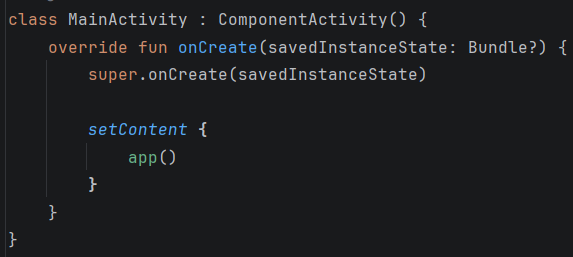
\includegraphics[width=0.85\textwidth]{Practica1_codigo1}
	\caption{Estructura inicial de MainActivity.}
	\label{fig:practica1codigo1}
\end{figure}

Posteriormente, se utilizó la anotación
\texttt{@Composable} para definir la función app(),
la cual contiene los elementos visuales de la
aplicación. También se agregó la anotación
\texttt{@Preview}, que permite visualizar una
representación de la interfaz directamente en
Android Studio durante el desarrollo.

\begin{figure}[H]
	\centering
	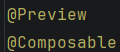
\includegraphics[width=0.85\textwidth]{Practica1_codigo2}
	\caption{Definición de la función composable y habilitación de la vista previa mediante @Preview.}
	\label{fig:practica1codigo2}
\end{figure}

A continuación, se implementó el componente
LazyColumn para organizar los elementos de la
interfaz de manera vertical. Mediante Modifier se
establecieron sus propiedades visuales, utilizando
fillMaxSize() para ocupar el espacio disponible
y background(Color.Gray) para establecer un
fondo de color gris.

\begin{figure}[H]
	\centering
	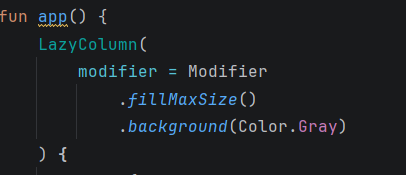
\includegraphics[width=0.85\textwidth]{Practica1_codigo3}
	\caption{Implementación de LazyColumn para organizar los elementos de la interfaz en una lista vertical desplazable.}
	\label{fig:practica1codigo3}
\end{figure}

En este fragmento se utiliza el componente Image de Jetpack Compose para insertar una imagen dentro de la interfaz de usuario. Mediante la propiedad modifier se configura su tamaño: fillMaxWidth() permite que la imagen ocupe todo el ancho disponible, mientras que height(400.dp) establece una altura de 400 unidades independientes de la densidad.

Por otra parte, la propiedad \texttt{painter} utiliza
\texttt{painterResource()} para cargar la imagen
almacenada en los recursos del proyecto, identificada
como \texttt{R.drawable.d\_cyberpunk}. Finalmente,
\texttt{contentDescription} proporciona una descripción
de la imagen, en este caso representada por el texto
\texttt{"D"}.

\begin{figure}[H]
	\centering
	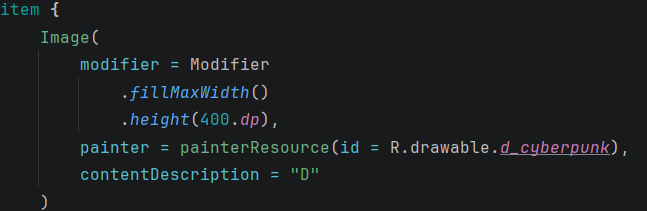
\includegraphics[width=0.85\textwidth]{Practica1_codigo4}
	\caption{Configuración del componente Image para mostrar una imagen y establecer sus dimensiones.}
	\label{fig:practica1codigo4}
\end{figure}

En este fragmento se implementa el componente \texttt{Text},
encargado de mostrar contenido textual dentro de la interfaz
de usuario. Mediante la propiedad \texttt{text} se establece
el mensaje \texttt{"Proyecto aplicaciones moviles"}.

La propiedad \texttt{fontSize} define el tamaño de la fuente
en 32 unidades independientes de la densidad (\texttt{sp}),
mientras que \texttt{color} establece el color de las letras
en blanco mediante \texttt{Color.White}.

Además, se utiliza \texttt{Modifier.fillMaxWidth()} para
hacer que el componente ocupe todo el ancho disponible y
\texttt{textAlign = TextAlign.Center} para centrar el texto
horizontalmente dentro del espacio asignado.

\begin{figure}[H]
	\centering
	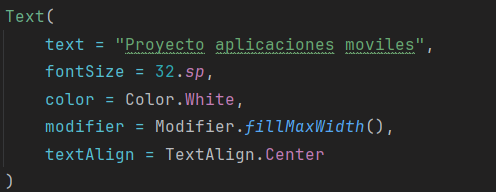
\includegraphics[width=0.85\textwidth]{Practica1_codigo5}
	\caption{Configuración del componente Text para mostrar un mensaje con tamaño, color y alineación personalizados.}
	\label{fig:practica1codigo5}
\end{figure}

En la siguiente figura se muestra el resultado de la
implementación de los componentes \texttt{Image} y
\texttt{Text} dentro de la interfaz de usuario. En la
parte superior se visualiza la imagen cargada desde
los recursos del proyecto, ocupando el ancho disponible
de la pantalla.

Debajo de la imagen se muestra el texto
\texttt{"Proyecto aplicaciones moviles"}, con un
tamaño de fuente de 32 \texttt{sp}, color blanco y
alineación centrada. También se observa el fondo de
color gris establecido mediante la propiedad
\texttt{background(Color.Gray)}.

Esta ejecución permite comprobar la correcta
visualización y distribución de los elementos
implementados en la interfaz de la aplicación.

\begin{figure}[H]
	\centering
	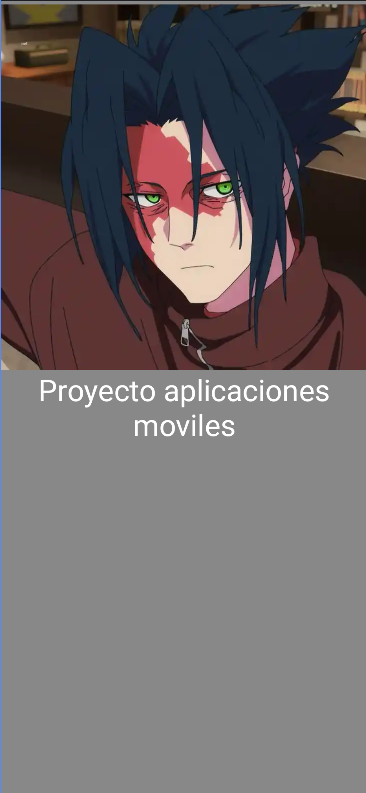
\includegraphics[width=0.45\textwidth]{Practica1_codigo6}
	\caption{Resultado de la implementación de los componentes Image y Text en el emulador de Android.}
	\label{fig:practica1codigo6}
\end{figure}

En esta figura se muestra la ejecución de la aplicación
en el emulador de Android, utilizando una representación
de un dispositivo móvil. En la parte superior de la
interfaz se visualiza la imagen cargada desde los
recursos del proyecto, ajustada al ancho disponible
de la pantalla.

Debajo de la imagen se presenta el texto
\texttt{"Proyecto aplicaciones moviles"}, con un
tamaño de fuente de 32 \texttt{sp}, color blanco y
alineación centrada. El resto de la interfaz conserva
el fondo de color gris establecido durante la
implementación.

También se pueden observar los elementos de navegación
y la barra de estado del dispositivo virtual, lo que
permite apreciar cómo se distribuye el contenido dentro
de una pantalla con formato de teléfono móvil.

\begin{figure}[H]
	\centering
	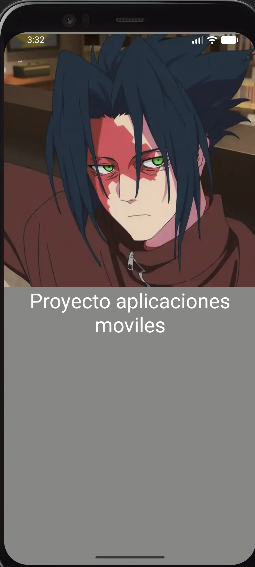
\includegraphics[width=0.45\textwidth]{Practica1_codigo7}
	\caption{Ejecución de la interfaz de usuario en el emulador de Android con formato de dispositivo móvil.}
	\label{fig:practica1codigo7}
\end{figure}

En esta figura se muestra el comportamiento de la
interfaz de usuario al cambiar la orientación del
dispositivo móvil de vertical a horizontal. Se puede
observar cómo los componentes visuales se ajustan
a las nuevas dimensiones de la pantalla, modificando
su distribución para aprovechar el espacio disponible.

La imagen se mantiene visible en la interfaz, mientras
que el texto \texttt{"Proyecto aplicaciones moviles"}
se adapta a la orientación horizontal del dispositivo.
Esto permite comprobar que la interfaz responde a los
cambios de orientación y se ajusta a las dimensiones
de la pantalla, proporcionando una visualización
adecuada tanto en formato vertical como horizontal.

\begin{figure}[H]
	\centering
	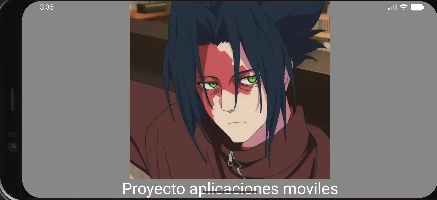
\includegraphics[width=0.85\textwidth]{Practica1_codigo8}
	\caption{Visualización de la interfaz en orientación horizontal, demostrando su adaptación al cambio de orientación del dispositivo móvil.}
	\label{fig:practica1codigo8}
\end{figure}

\subsubsection{Resultados}
Como resultado de esta práctica, se logró implementar
una interfaz de usuario mediante Jetpack Compose,
utilizando los componentes \texttt{Column} y
\texttt{LazyColumn} para organizar los elementos
visuales de manera vertical.

Se consiguió incorporar una imagen y un texto dentro
de la interfaz mediante los componentes
\texttt{Image} y \texttt{Text}, configurando sus
propiedades para modificar sus dimensiones, tamaño
de fuente, color y alineación.

Durante las pruebas realizadas en el emulador de
Android, se comprobó la correcta visualización de
los elementos tanto en orientación vertical como
horizontal. Esto permitió observar cómo cambia la
distribución del contenido al modificar la
orientación del dispositivo.

Finalmente, la práctica permitió comprender el uso
de los componentes de Jetpack Compose para construir
interfaces, así como la importancia de configurar
adecuadamente sus propiedades visuales para obtener
una presentación organizada del contenido.

\subsection{Practica 3. Filas en Jetpack Compose}

\subsubsection{Introducción}
En esta práctica se aborda el uso de filas mediante Jetpack Compose, una herramienta que permite organizar y distribuir los elementos de una interfaz de usuario en aplicaciones Android. Se estudia el funcionamiento de los componentes Row y LazyRow, los cuales permiten colocar elementos de manera horizontal y facilitan la distribución del contenido dentro de una pantalla.

Durante el desarrollo se implementan diferentes elementos de texto dentro de una fila, utilizando propiedades de organización horizontal para establecer la separación y distribución de los componentes. Asimismo, se emplean modificadores para configurar el ancho y el espaciado de los elementos, permitiendo adaptar su presentación dentro de la interfaz.

También se utiliza LazyRow para mostrar contenido en una lista horizontal desplazable, mientras que LazyColumn permite organizar los elementos de manera vertical. De esta forma, se busca comprender cómo funcionan ambos componentes y cómo pueden combinarse para construir interfaces que permitan recorrer su contenido.
\subsubsection{Herramientas y tecnologías utilizadas}
\begin{itemize}
	
	\item \textbf{Android Studio:} Entorno de desarrollo integrado (IDE) utilizado para crear, editar y ejecutar el proyecto de aplicación Android.
	
	\item \textbf{Kotlin:} Lenguaje de programación empleado para escribir el código de la aplicación y definir las funciones que construyen la interfaz.
	
	\item \textbf{Jetpack Compose:} Conjunto de herramientas de Android utilizado para desarrollar interfaces de usuario mediante funciones composables.
	
	\item \textbf{Row:} Componente de Jetpack Compose que permite organizar los elementos de una interfaz de manera horizontal.
	
	\item \textbf{LazyRow:} Componente utilizado para mostrar elementos en una lista horizontal desplazable, facilitando la visualización de contenido que supera el ancho disponible de la pantalla.
	
	\item \textbf{LazyColumn:} Componente que permite organizar elementos verticalmente y recorrer el contenido mediante desplazamiento.
	
	\item \textbf{Arrangement:} Propiedad utilizada para controlar la distribución y separación de los elementos dentro de una fila.
	
	\item \textbf{Modifier:} Herramienta que permite configurar las propiedades de los componentes, como sus dimensiones, espaciado y apariencia visual.
	
	\item \textbf{Android Emulator:} Dispositivo virtual integrado en Android Studio, utilizado para ejecutar la aplicación y observar el resultado de la interfaz.
	
\end{itemize}
\subsubsection{Procedimiento}
En primer lugar, se implementó el componente Row de
Jetpack Compose con el propósito de organizar
diferentes elementos de texto de manera horizontal.
Dentro de este componente se agregaron tres elementos
mediante Text, correspondientes a las etiquetas
``Stack:'', ``C++'' y ``Kotlin''. También se estableció
el color blanco para el contenido de los textos.

\begin{figure}[H]
	\centering
	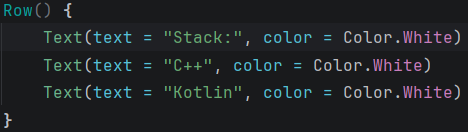
\includegraphics[width=0.85\textwidth]{Practica2_codigo1}
	\caption{Implementación del componente Row para organizar elementos de texto de manera horizontal.}
	\label{fig:practica2codigo1}
\end{figure}

Posteriormente, se modificó la estructura de Row
incorporando la propiedad horizontalArrangement con
el valor Arrangement.SpaceEvenly. Esta propiedad
permite distribuir los elementos de manera uniforme
dentro del espacio disponible. Asimismo, se utilizó
Modifier.fillMaxWidth() para ocupar el ancho de la
pantalla y padding(all = 16.dp) para establecer un
espaciado alrededor de la fila.

\begin{figure}[H]
	\centering
	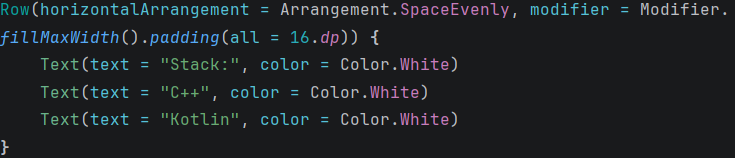
\includegraphics[width=0.85\textwidth]{Practica2_codigo2}
	\caption{Configuración de Row mediante Arrangement.SpaceEvenly y Modifier para distribuir los elementos horizontalmente.}
	\label{fig:practica2codigo2}
\end{figure}

Posteriormente, se incorporó el componente LazyRow
para organizar diferentes elementos de texto en una
lista horizontal. Dentro de este componente se
utilizó la propiedad horizontalArrangement para
configurar la distribución del contenido, así como
Modifier.fillMaxWidth() y padding() para establecer
el ancho y el espaciado de la fila.

Mediante LazyRow se integraron diferentes nombres
de lenguajes de programación y tecnologías, como
C++, Kotlin, Java, PHP, Python, C\# y JavaScript.
Este componente permite recorrer horizontalmente
el contenido cuando supera el espacio disponible
en la pantalla.

\begin{figure}[H]
	\centering
	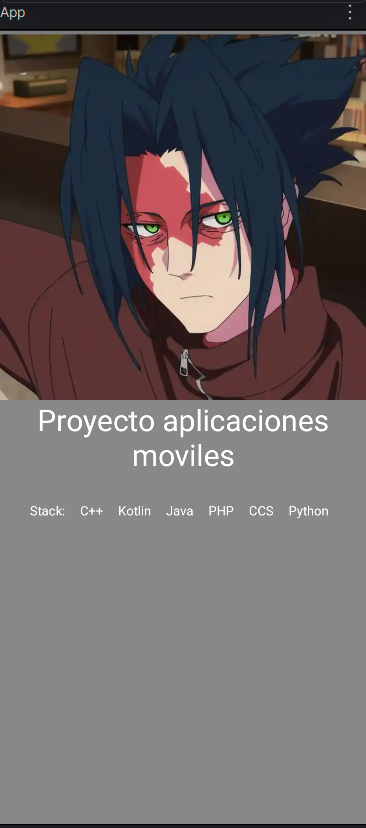
\includegraphics[width=0.45\textwidth]{Practica2_codigo3}
	\caption{Visualización de LazyRow con elementos distribuidos horizontalmente en orientación vertical}
	\label{fig:practica2codigo3}
\end{figure}



Finalmente, se ejecutó la aplicación para observar
el resultado de la implementación. Se comprobó que
los elementos de texto se muestran horizontalmente
dentro de la interfaz, junto con la imagen y el título
previamente incorporados.

\begin{figure}[H]
	\centering
	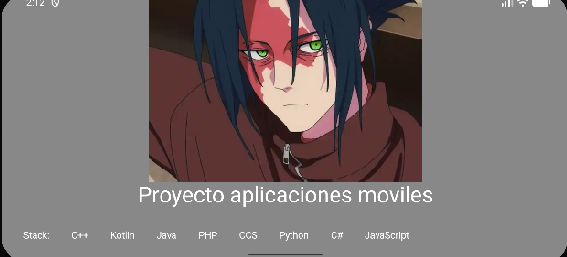
\includegraphics[width=0.85\textwidth]{Practica2_codigo4}
	\caption{Adaptación de la interfaz y visualización de LazyRow en orientación horizontal}
	\label{fig:practica2codigo5}
\end{figure}



\subsubsection{Resultados}
Como resultado de esta práctica, se obtuvo una interfaz de usuario que integra elementos organizados tanto vertical como horizontalmente mediante los componentes LazyColumn y LazyRow de Jetpack Compose.

La interfaz muestra una imagen en la parte superior, seguida de un título centrado y una fila de textos que representa diferentes elementos relacionados con lenguajes de programación. También se comprobó la utilidad de las propiedades de distribución y espaciado para organizar los componentes dentro de la pantalla.

Con esta implementación se comprendió la diferencia entre Row y LazyRow, así como su combinación con LazyColumn para construir interfaces que permiten organizar y recorrer contenido en diferentes direcciones.

\newpage

\subsection{Practica 4. States en Jetpack Compose}

\subsubsection{Introducción}
En esta práctica se aborda el manejo de estados mediante Jetpack Compose, un conjunto de herramientas que permite desarrollar interfaces de usuario para aplicaciones Android. Se estudia el funcionamiento de los estados y su utilización para almacenar valores que pueden modificarse durante la ejecución de una aplicación.

Durante el desarrollo se implementa una variable denominada counter, utilizando mutableStateOf() para establecer un valor inicial y remember para conservar su estado durante las recomposiciones de la interfaz. Posteriormente, se emplea rememberSaveable para mantener el valor almacenado cuando se producen cambios en la configuración del dispositivo.

Asimismo, se utiliza el componente Text para mostrar el valor de la variable dentro de la interfaz, permitiendo observar cómo se refleja el estado en la pantalla. El propósito de esta práctica es comprender la importancia de los estados en Jetpack Compose y conocer algunas de las herramientas disponibles para administrarlos.

\subsubsection{Herramientas y tecnologías utilizadas}

\begin{itemize}
	
	\item \textbf{Android Studio:} Entorno de desarrollo integrado (IDE) utilizado para crear, editar y ejecutar el proyecto de aplicación Android.
	
	\item \textbf{Kotlin:} Lenguaje de programación empleado para escribir el código de la aplicación y declarar las variables utilizadas en la interfaz.
	
	\item \textbf{Jetpack Compose:} Conjunto de herramientas de Android utilizado para desarrollar interfaces de usuario mediante funciones composables.
	
	\item \textbf{State:} Mecanismo utilizado para almacenar información que puede cambiar durante la ejecución de la aplicación y actualizar la interfaz cuando se modifica su valor.
	
	\item \textbf{mutableStateOf():} Función que permite crear un estado observable y establecer un valor inicial.
	
	\item \textbf{remember:} Función que permite conservar un valor durante las recomposiciones de una función composable.
	
	\item \textbf{rememberSaveable:} Función que permite conservar y restaurar el estado cuando se producen cambios de configuración, como la rotación del dispositivo.
	
	\item \textbf{Text:} Componente utilizado para mostrar el valor almacenado en la variable de estado dentro de la interfaz.
	
	\item \textbf{Android Emulator:} Dispositivo virtual utilizado para ejecutar la aplicación y comprobar la visualización de los estados en diferentes orientaciones.
	
	\item \textbf{clickable():} Modificador de Jetpack Compose que permite detectar interacciones de clic o pulsación sobre un componente y ejecutar una acción.
	
\end{itemize}

\subsubsection{Procedimiento}
En primer lugar, se incorporó un componente Row para organizar horizontalmente una imagen de favorito y un elemento de texto que muestra un valor numérico. Para representar el icono se utilizó un recurso vectorial dentro de la carpeta drawable del proyecto.

\begin{figure}[H]
	\centering
	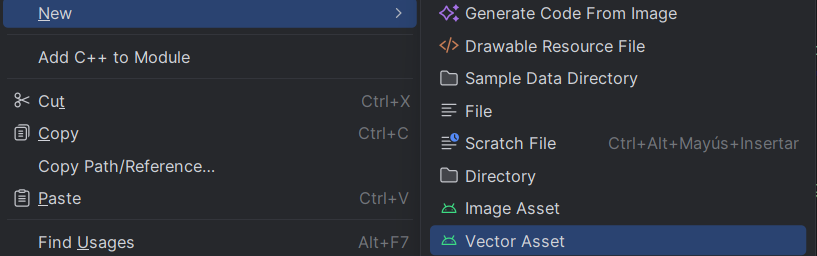
\includegraphics[width=0.85\textwidth]{Practica3_codigo1}
	\caption{Creación de un nuevo asset en la carpeta drawable}
	\label{fig:practica3codigo1}
\end{figure}

Posteriormente, se creó el recurso gráfico mediante la herramienta Vector Asset de Android Studio, seleccionando un icono de corazón. El archivo generado se almacenó con el nombre favorite1.xml, permitiendo utilizarlo dentro de la interfaz mediante painterResource()

\begin{figure}[H]
	\centering
	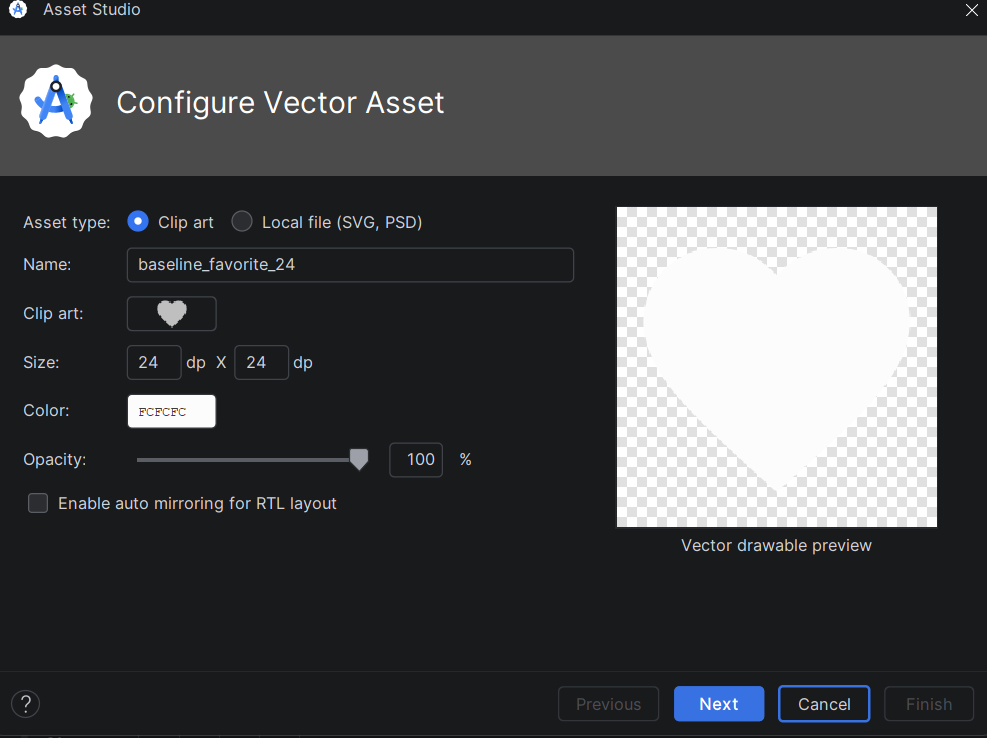
\includegraphics[width=0.85\textwidth]{Practica3_codigo2}
	\caption{Creación del nuevo asset favorite1}
	\label{fig:practica3codigo2}
\end{figure}

Despues de crear el vertical asset en la carpeta drawable se tiene una nueva figura para utilizarla en nuestro proyecto

\begin{figure}[H]
	\centering
	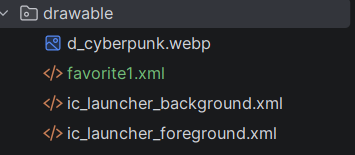
\includegraphics[width=0.85\textwidth]{Practica3_codigo3}
	\caption{Vertical asset en la carpeta drawable}
	\label{fig:practica3codigo3}
\end{figure}

Para poder hacer uso de esta imagen se creo el componente row y se imprimio el asset favorite1 que se mostrara en el simulador 

\begin{figure}[H]
	\centering
	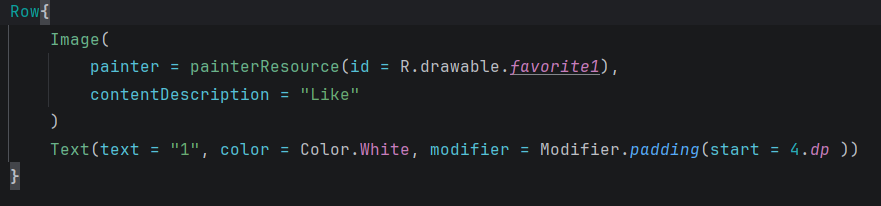
\includegraphics[width=0.85\textwidth]{Practica3_codigo4}
	\caption{Vertical asset en la carpeta drawable}
	\label{fig:practica3codigo4}
\end{figure}

Se modifico la columna para que pudiera tener un modifier para modificar la estructura del asset y poder moverla de posicion, en este caso en la parte de abajo de la imagen 

\begin{figure}[H]
	\centering
	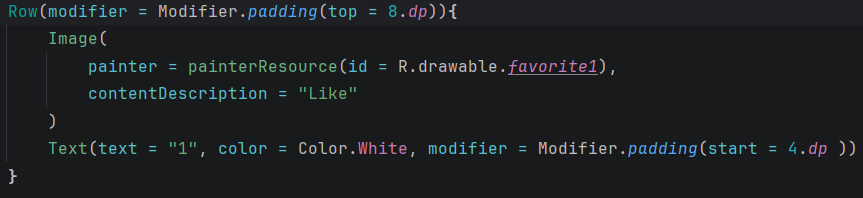
\includegraphics[width=0.85\textwidth]{Practica3_codigo5}
	\caption{Vertical asset en la carpeta drawable}
	\label{fig:practica3codigo5}
\end{figure}

Asimismo se muestra en el simulador el como quedo el resultado despues de aplicar el modificador en el simulador 

\begin{figure}[H]
	\centering
	
\includegraphics[width=0.45\textwidth]{Practica3_codigo6}
	\caption{Verificacion de la creación del asset favorite1}
	\label{fig:practica3codigo6}
\end{figure}

A continuación, se agregó una variable denominada counter dentro de la función App(), utilizando remember y mutableStateOf(0) para establecer un estado inicial con valor cero. También se incorporaron las importaciones necesarias para utilizar estas funciones, incluyendo mutableStateOf, remember y getValue.



Posteriormente, se agregó la propiedad clickable() al
modificador de la imagen del corazón, permitiendo
detectar las interacciones del usuario. Dentro de
esta propiedad se implementó la instrucción
counter++, la cual incrementa en una unidad el
valor almacenado en la variable counter cada vez
que se presiona la imagen.

Debido a que counter es una variable de estado,
la modificación de su valor provoca una
recomposición de la interfaz, actualizando el
número que se muestra junto al icono del corazón.

Después, se modificó el componente Text que inicialmente mostraba un valor fijo de uno. En su lugar, se utilizó counter.toString() para representar el valor almacenado en la variable de estado y mostrarlo dentro de la interfaz.

Posteriormente, se modificó la declaración de la variable counter, sustituyendo val por var. Este cambio permite modificar el valor de la variable durante la ejecución de la aplicación, manteniendo su declaración mediante remember y mutableStateOf().

Finalmente, se sustituyó remember por rememberSaveable, conservando mutableStateOf(0) como valor inicial. Con esta modificación se busca mantener el estado almacenado ante cambios de configuración del dispositivo. Se ejecutó la aplicación en el emulador para comprobar la visualización del valor y observar su comportamiento al cambiar la orientación de la pantalla.

\subsubsection{Resultados}
Como resultado de esta práctica, se implementó un mecanismo de almacenamiento de estados mediante las funciones mutableStateOf(), remember y rememberSaveable de Jetpack Compose.

Se consiguió mostrar un valor numérico junto a un icono de corazón dentro de la interfaz de usuario. Durante las pruebas se observaron diferentes valores del contador, incluyendo el valor inicial de cero y un valor posterior de cinco.

También se comprobó la presentación de la interfaz en orientación vertical y horizontal, utilizando rememberSaveable para conservar el estado ante cambios de configuración del dispositivo.

Mediante esta práctica se comprendió cómo se pueden declarar y utilizar variables de estado en Jetpack Compose, así como la importancia de estos mecanismos para mantener actualizada la información mostrada en una aplicación Android.


\end{document}

